\section{问题重述}

\subsection{研究背景}

世界杯小组赛的组织并非单一的赛程排列问题。赛事关注度决定转播与票务需求，比赛安排又同时受到场馆容量、时区、球队休息、安保能力和转播资源的约束；进入比赛阶段以后，前两轮赛果还会改变第三轮的晋级形势、需求强度与风险水平。因此，组织者真正需要的是一条从赛前预测延伸到赛中调整、并能够与现实赛程比较的完整决策链。

题目给出由48支球队、12个小组和72场比赛构成的模拟世界杯。每组4队进行单循环赛，每队参加3场；每组前2名直接晋级，12个第三名中排名靠前的8队补足32强。候选资源包括16个场馆和80个参考时段，赛程必须满足唯一指派、相邻两轮至少60小时、场馆逐日与总负荷、黄金时段公平、安保资格以及同一时段转播容量等规则。

\subsection{四个子问题}

问题一要求在题定时间划分下预测转播观看人数。训练集560场、测试集140场，测试标签不可用于任何训练或调参；对历史赛后信息只能构造严格滞后的赛前统计。模型既要输出测试集百万人尺度预测，也要为72场模拟小组赛给出人尺度预测，从而为后续传播价值计算提供输入。

问题二需要同时确定每场比赛的场馆和开球时段。优化对象不是先选场馆、再向空闲时段填充，而是比赛、场馆、时段的联合指派；目标综合票务、传播、悬念、吸引力、成本、旅行、公平与风险八个维度。除给出综合目标值外，最终方案还须逐项通过赛程规则复算，才能称为可执行排程。

问题三固定问题二得到的第三轮场馆与时段，仅根据前两轮反馈重新配置转播优先级、安保等级、交通保障和票价。24场第三轮比赛共享同一信息截面，并在20,000次联合比分模拟中统一处理组内排名与跨组第三名竞争。动态方案需与赛前已经优化并锁定的静态方案在相同动作域、相同日约束和相同归一化边界下比较，以识别信息更新带来的真实增益。

问题四选取一届已结束的四队小组制世界杯，将实际小组赛与本文72场优化方案放入同一评价函数。由于两项赛事分别有48场和72场，票务、传播、成本、旅行与风险等总量必须先转换为场均强度。现实数据中的商业和安保字段无法直接观测时，应把代理指标与可观测结构分层报告，不用代理综合分数替代对现实组织约束的判断。

\subsection{总体研究路线}

四问之间存在明确的输入输出关系：问题一提供赛前观看需求，问题二把需求转化为场馆时段排程；问题三读取该排程的第三轮部分，问题四则复用问题二的评价口径。围绕这条链路，本文先冻结数据与单位口径，再进行预测、联合优化、动态重配置和现实比较，最后统一开展约束审计与敏感性检验。整体步骤及各阶段交付见图\ref{fig:roadmap}。

\begin{figure}[htbp]
\centering
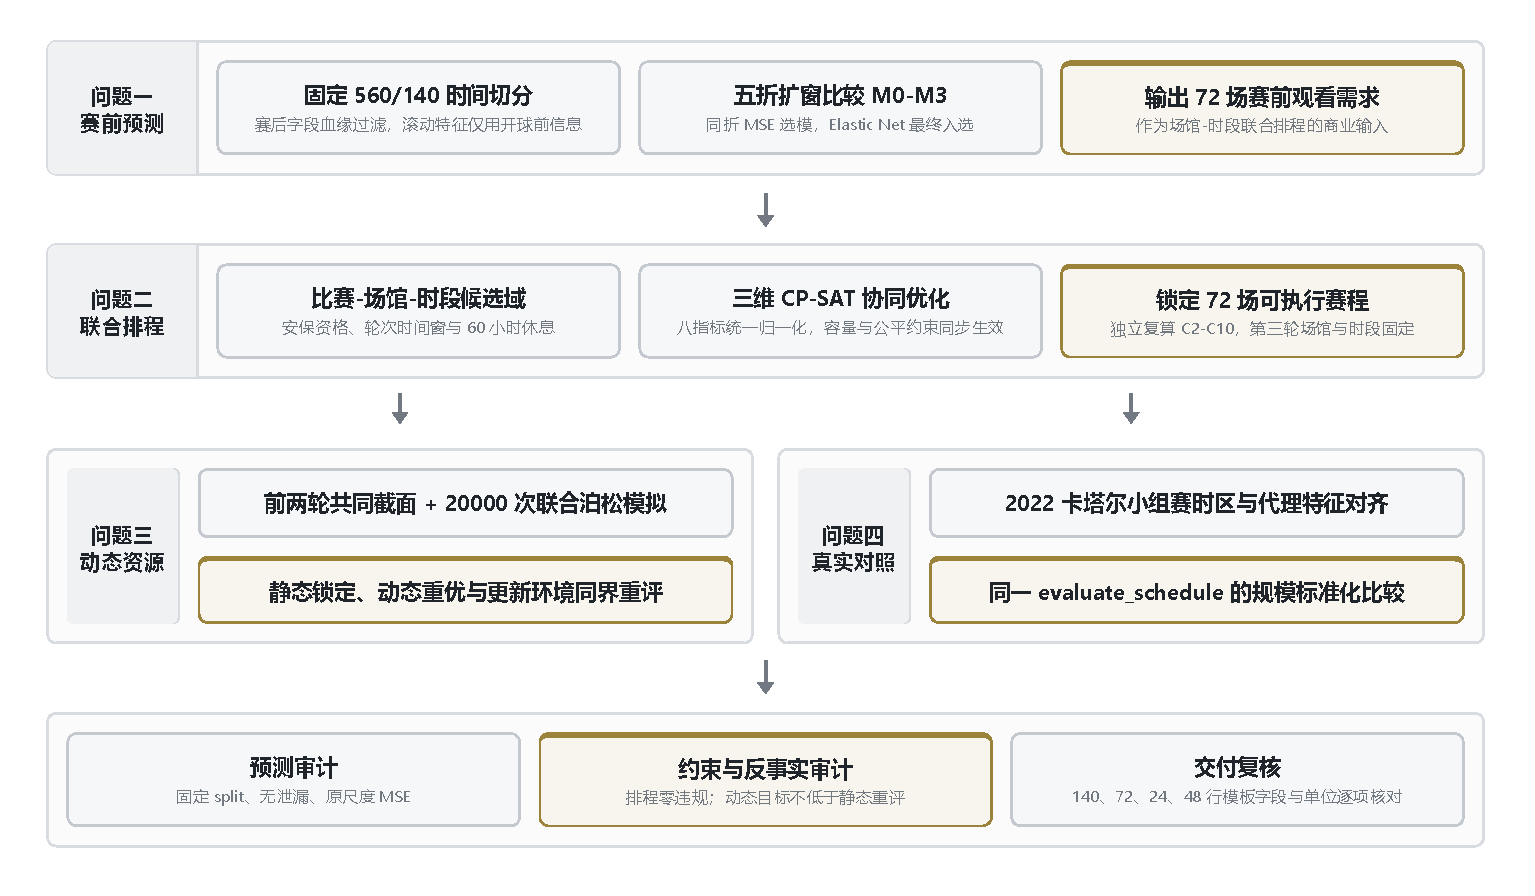
\includegraphics[width=0.85\textwidth,height=0.7\textheight,keepaspectratio]{../figures/fig_roadmap.pdf}
\caption{整体技术路线图}\label{fig:roadmap}
\end{figure}

数据合同与约束审计贯穿全部四问，而不是仅在求解结束后补做检查（见图\ref{fig:roadmap}）。预测结果以两种单位导出，排程结果以72行物理方案保存，动态策略以24场动作保存，实际赛程以48行长表保存；这种逐层固化使后续模型能够直接追溯上游输入。最终评价只复用已经定义的指标和方向，避免为迎合某个方案而重新选择分母或归一化边界。
